%!TEX root = ../main.tex
\subsection{ECAL Calibrations}

The energy $E$ deposited in each electromagnetic calorimeter (ECAL) crystal is reconstructed according to 
\[
E = A \cdot G \cdot LC(t) \cdot C(t),
\]
where
$A$ is the digital signal amplitude above the \emph{pedestals},
$G$ is a conversion factor from ADC counts to \GeV,
$LC(t)$ are the \emph{laser corrections} that account for the effect of irradiation of the crystals due to the LHC collisions, and
$C(t)$ is a combinations of calibration constants that account for the different crystal and photodetector responses, \textit{i.e.} the \emph{intercalibrations}.
These aim to equalise the ECAL response both for different crystals at the same $\eta$ coordinate,
and
the absolute scale as a function of $\eta$.
Finally, the measurement of the electronic \emph{pulse shapes} themselves is also paramount to the ECAL calibration, not only for the measurement of the deposit energy but also for the \emph{timing capabilities} of the subdetector.
A more detailed description of
the operation and performance of the CMS ECAL,
including calibration procedures,
is available in Ref.~\cite{CMS:2024ppo}.

%%% I don't know how much I believe these numbers here.
Out of the 326 conditions in the HLT GT,
67 are related to ECAL, %59
of which 52 are relevant to \Runthree data-taking. %36
From these, the following are considered core and critical for data-taking:
\begin{table}[h!]
    \centering
    \begin{adjustbox}{max width=\textwidth}
    \begin{tabular}{p{3.5cm}|p{4.5cm}|p{2.5cm}|p{2cm}|p{4cm}}
        \textbf{Name} & \textbf{Record} & \textbf{Workflow} & \textbf{Frequency of Updates} & \textbf{Description} \\ \hline
    Laser corrections & \texttt{EcalLaserAPDPNRatios} & ECAL automation and manual & Every 40 min or per fill & Crystal transparency and photodetector response. \\
    Pedestals & \texttt{EcalPedestals} & PCL and ECAL automation & Per run or weekly & Pedestals for noise measurements. \\
    Pulse shapes & \texttt{EcalPulseShapes} & ECAL automation and manual & 3 days & Pulse shapes. \\
    Timing & \texttt{EcalTimeCalibConstants} & ECAL automation and manual & Weekly & Time of the pulse maximum.\\
    Intercalibrations & \texttt{EcalIntercalibConstants} & ECAL automation and manual & Weekly or more & Equalise crystal response vs. $\eta$ and $\phi$.
    \end{tabular}
    \end{adjustbox}
    \caption{Fundamental ECAL Calibrations, ordered in terms of frequency of updates.}
    \label{tab:ECALCalibrations_critical}
\end{table}

\subsubsection{Pedestals}

%EcalPedestalsRcd

The ECAL pedestals represent the baseline from which the electronics pulses are measured.
Pedestals are measured for the three possible configurations (gains) of the multi-gain preamplifier integrated in the ECAL readout chip: $\times 1$, $\times 6$ and $\times 12$.
In the offline tag,
the PCL updates the G12 pedestals automatically, while
the G1 and G6 pedestals are updated manually every week.
In the online tag, all three pedestals are updated manually weekly.

\subsubsection{Laser Corrections}

%EcalLaserAPDPNRatiosRcd

The transparency of the ECAL crystals and the photodetector's response to light are degraded as an effect of the irradiation from the LHC collisions.
The degradation as a function of time is monitored crystal by crystal by measuring the response to the light of a laser system.
The light is injected in the system during the LHC abort gap, and a complete scan of the calorimeter takes 40 minutes.
The measurement of the response degradation is then used as a correction factor in the energy reconstruction.
In the offline tag, this correction is available with that same 40-minutes granularity,
while in the online tag it is available only once per LHC fill.
Figure~\ref{fig:ECALTransparency} shows the ECAL relative response to the laser light,
as a function of time,
for the LHC \Runtwo.
We can see that the more forward sections of the subdetector show the largest response decrease as expected, due to the strongest irradiation to which they're subjected.
\begin{figure}[htbp]
   \centering
   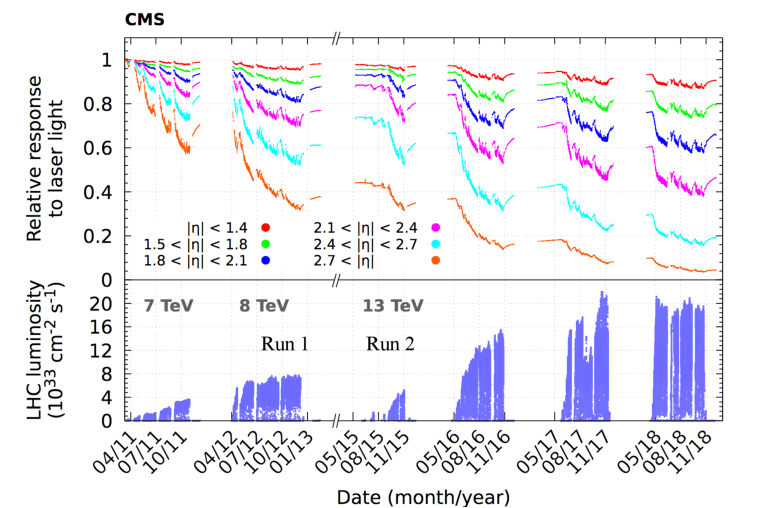
\includegraphics[width=0.7\textwidth]{figures/ECALTransparencyEvolutionRun2.pdf}
   \caption{ECAL relative response to the laser light, as a function of time, for the LHC \Runtwo.
   The LHC instantaneous luminosity is also shown in the lower panel.
   Figure extracted from Ref.~\cite{CMS:2024ppo}.
}
   \label{fig:ECALTransparency}
\end{figure}

\subsubsection{Pulse Shapes}

%EcalPulseShapesRcd

The ECAL pulse shapes also change because of the irradiation affects,
and those changes also directly change the reconstruction of the signal amplitude.
These updates are more critical after a technical stop of the LHC.
The same payloads are used in the offline and online tags.

\subsubsection{Timing Corrections}

%EcalTimeCalibConstantsRcd

The fast signal from the crystal scintillation enables the ECAL subdetector to provide timing measurements in addition to energy.
In test beam conditions, the ECAL barrel achieved a 100\,ps precision for energy deposits above 10--20\GeV.
Effects from clock distribution variance,
instabilities in clock initialisation in different readout units,
and crystal degradation
decrease that precision to 180--350\,ps range.
The ECAL timing drifts
towards negative times during collisions
and
towards positive times during recovery.
For the current standard used for the calibration (ratio timing),
the same payloads are used in the offline and online tags.

\subsubsection{Intercalibrations}

%EcalIntercalibConstantsRcd

The intercalibrations are derived for each crystal and employ a series of methods:
the azimuthal symmetry of the energy deposits in ECAL,
the known mass of particles that decay to electrons and photons
($\text{Z}\to\text{ee}$, $\pi^0\to\gamma\gamma$),
and
the energy--momentum ratio ($E/p$) of electrons from electroweak boson decays.
In general these calibrations require multiple inverse femtobarns of integrated luminosity to derive;
the same payloads are used in the offline and online tags.

\subsubsection{Alignment}

Alignment of the ECAL with respect to the Tracker system is done infrequently,
mainly when there is a cycle of the CMS magnet.
We will not consider alignment conditions for subdetectors other than the Tracker for further discussion in this report.

\subsubsection{Recommendations}

In view of the above discussion, we consider the \emph{laser corrections} a possible candidate for the implementation in NGT.
The gap between online and offline update frequencies (40 minutes vs. per fill) is large enough that, in principle, expressive improvements can be realised by improving the online calibration.
